\chapter{MARP: Model Mappings for Analog Accelerators with Rectangular Packing}

MARP is a DNN mapper that can optimize the mapping of multiple layers in AIMC accelerators with interlayer weight reuse. We build MARP on the idea of using rectangular bin packing algorithms to pack multiple DNN layers into a single matrix written into the AIMC. We show that compared to naive single-mapping, utilizing MARP increases the utilizations of the MLPerfTiny models. On anomaly detection with the FC-AE model, MARP increased the utilization from 28.79\% to 80.63\%. On keyword spotting with the DS-CNN model, MARP increased the utilization from 5.01\% to 30.08\%. On image classification with the MobileNetV2 model, MARP increased the utilization from 35.85\% to 81.57\%. On image classification with the 3-block ResNet model, MARP increased the utilization from 9.95\% to 74.64\%.

Just as importantly, MARP reduces the number of AIMC cores needed to fully map models. MARP was able to reduce the number of AIMC cores needed to fully map the MobileNetV2 model from 91 in naive single-mapping to 34 in MARP. This is significant as AIMC accelerators like NeuRRAM \cite{wanneurram} has 48 cores which would not have been enough to fully map the MobileNetV2 model without eviction. With MARP, we can fully map the MobileNetV2 model without eviction and with high AIMC memory utilization.

The code for MARP is available at \url{https://github.com/Lawrence-lugs/hwacc_design_garage} and the specific compiler for QRAcc can be found in \url{https://github.com/Lawrence-lugs/QrAccelerator/blob/main/tests/stim_lib/compile.py}

\label{chapter:marp}

\section{Background: Rectangular Packing}

The rectangular packing problem is a well-known NP-hard problem in combinatorial optimization \cite{jylanki2010thousand}. It involves packing a set of rectangles into a larger rectangle (known as a bin) such that the total area of the rectangles is maximized while minimizing wasted space. Significant previous work has been done on trying find optimal solutions to the rectangular packing problem since it's relevant to many real-world applications such as loading cargo into trucks, packing boxes into containers, and cutting fabric or metal sheets. 

MARP is built on the idea that, in the context of DNN mappings, different subtypes of the rectangular packing problem can be used to map multiple DNN layers into a single AIMC memory array to maximize utilization or minimize the total write energy used by model inference. By treating each DNN layer as a rectangle and the AIMC memory array as a larger rectangle, we can use rectangular packing algorithms to find the optimal arrangements of DNN layers in the AIMC memory array.

\begin{figure}[htbp]
    \centering
    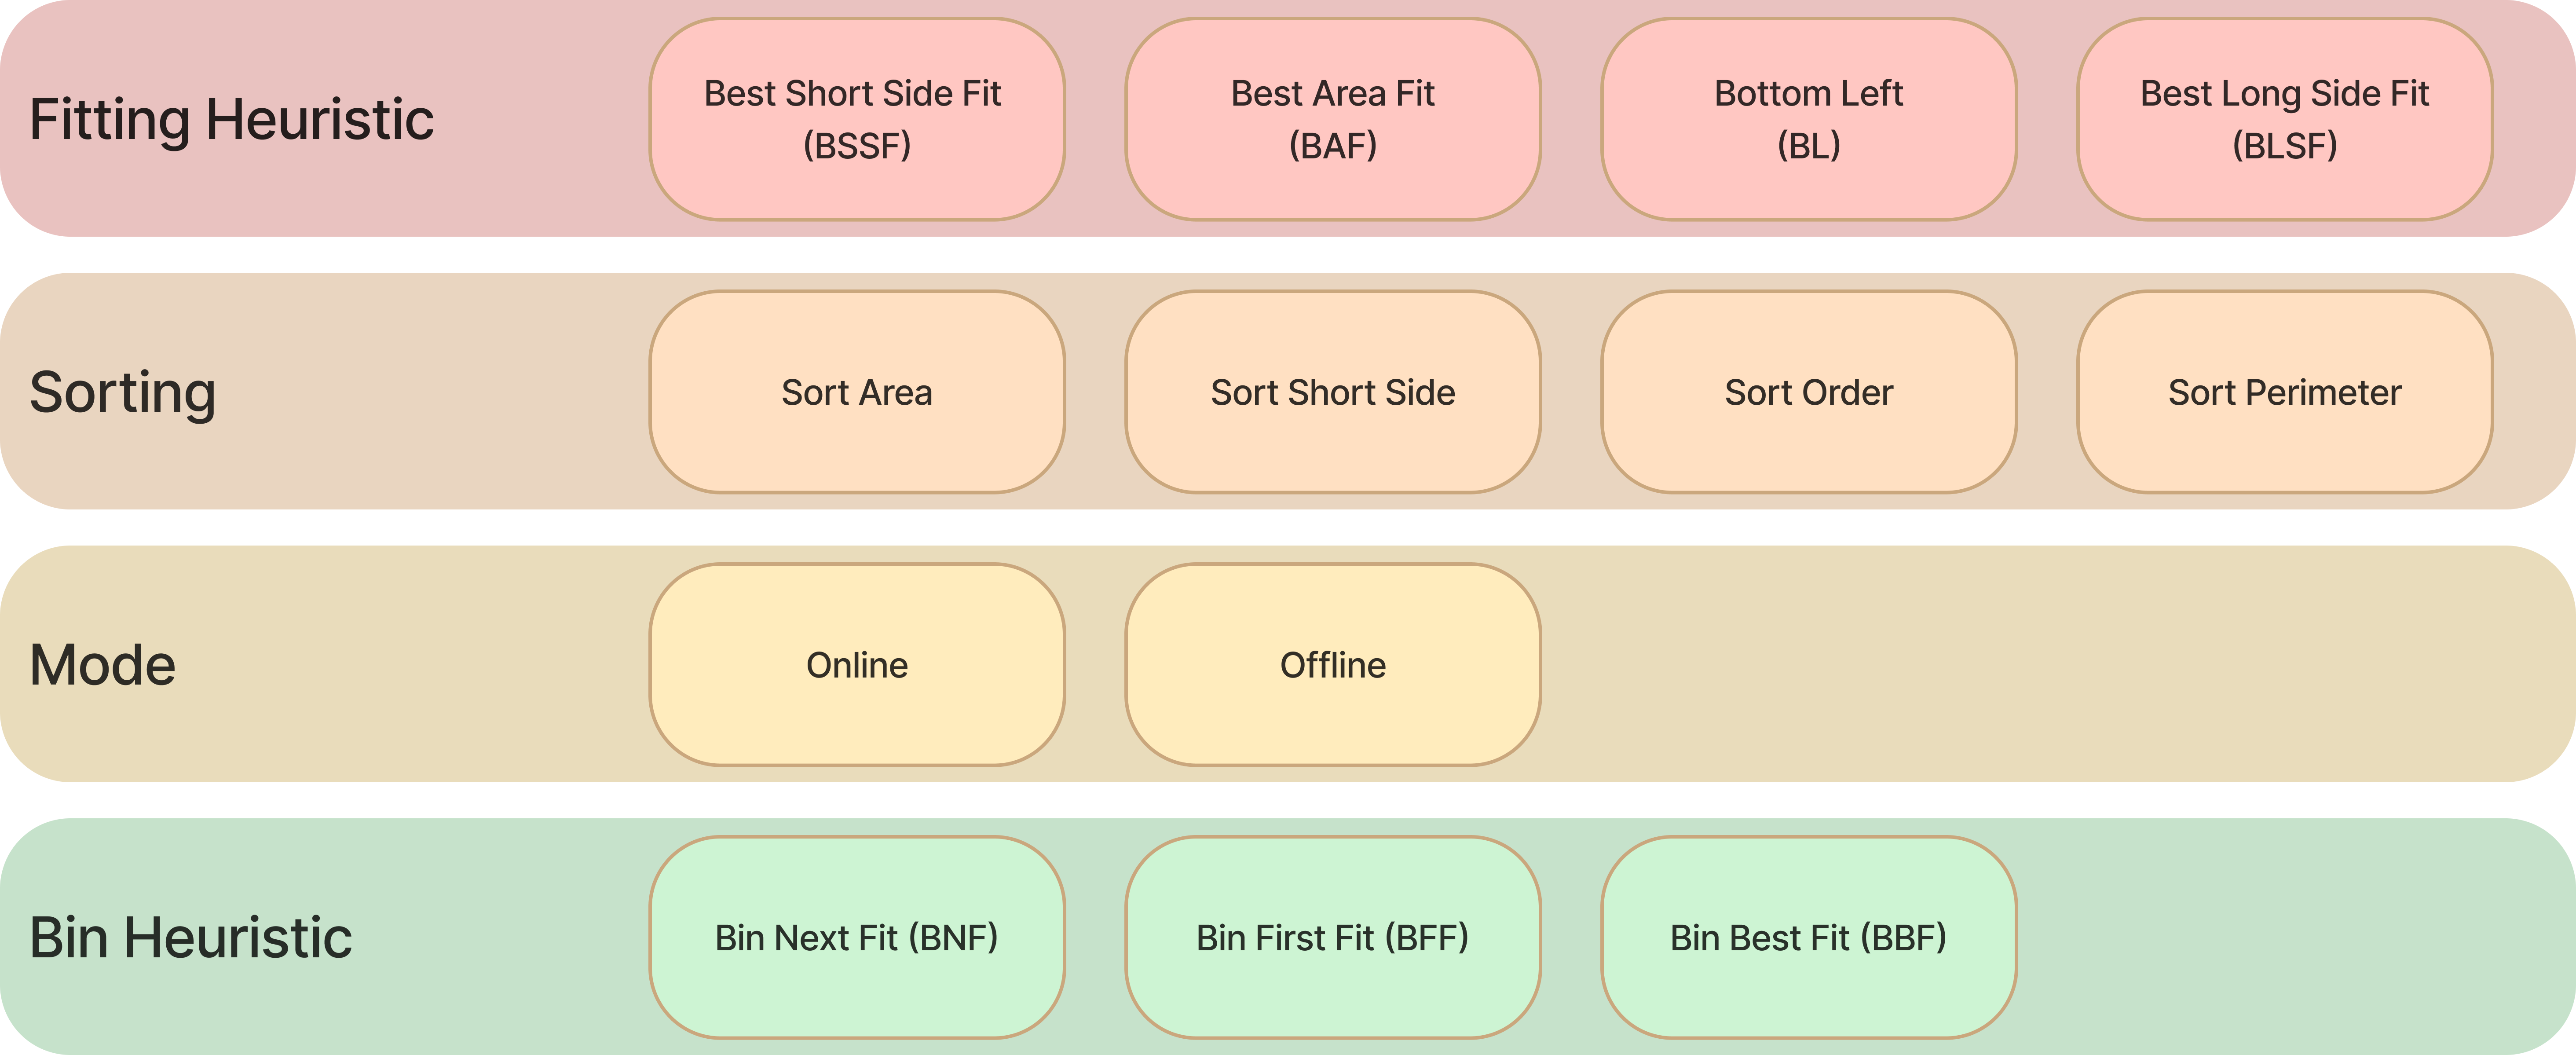
\includegraphics[width=\textwidth]{images/marp/rectpack_heuristics.png}
    \caption{Maximal Rectangles algorithm variants. For an in-depth explanation on more of the algorithm, see \cite{jylanki2010thousand}.}
    \label{fig:maximal_rectangles_variants}
\end{figure}

As of today, the most popular method of solving the general rectangular packing problem is the Maximal Rectangles (MaxRects) set of algorithms. Several variants of the Maximal Rectangles algorithm exist, as summarized in Figure \ref{fig:maximal_rectangles_variants}. Another method is the Skyline algorithm. The Skyline algorithm works faster than the MaxRects algorithm, but it is not as effective in terms of packing density \cite{jylanki2010thousand}. Lastly, there's also the Guillotine algorithm that specialized in creating packings that have straight edges that are easy to cut as much as possible. The Guillotine algorithms are useful for cutting sheets of material, but also are not as effective in terms of packing density as the MaxRects algorithm.  

For MARP, we find that the MaxRects algorithm is most effective in terms of packing density and we found that its variants tend to work well for DNN mapping. However, as user input, MARP allows any packer variants from the rectpack python library. Additionally, we implemented a naive single-mapping packer that simply maps each layer to a separate bin in the AIMC memory array to imitate the mappings of existing DNN mappers. We use the naive packer to compare the performance of MARP against the existing DNN mappers that do not use multi-mapping.

\subsection{MaxRects Algorithm}

\begin{figure}[htbp]
    \centering
    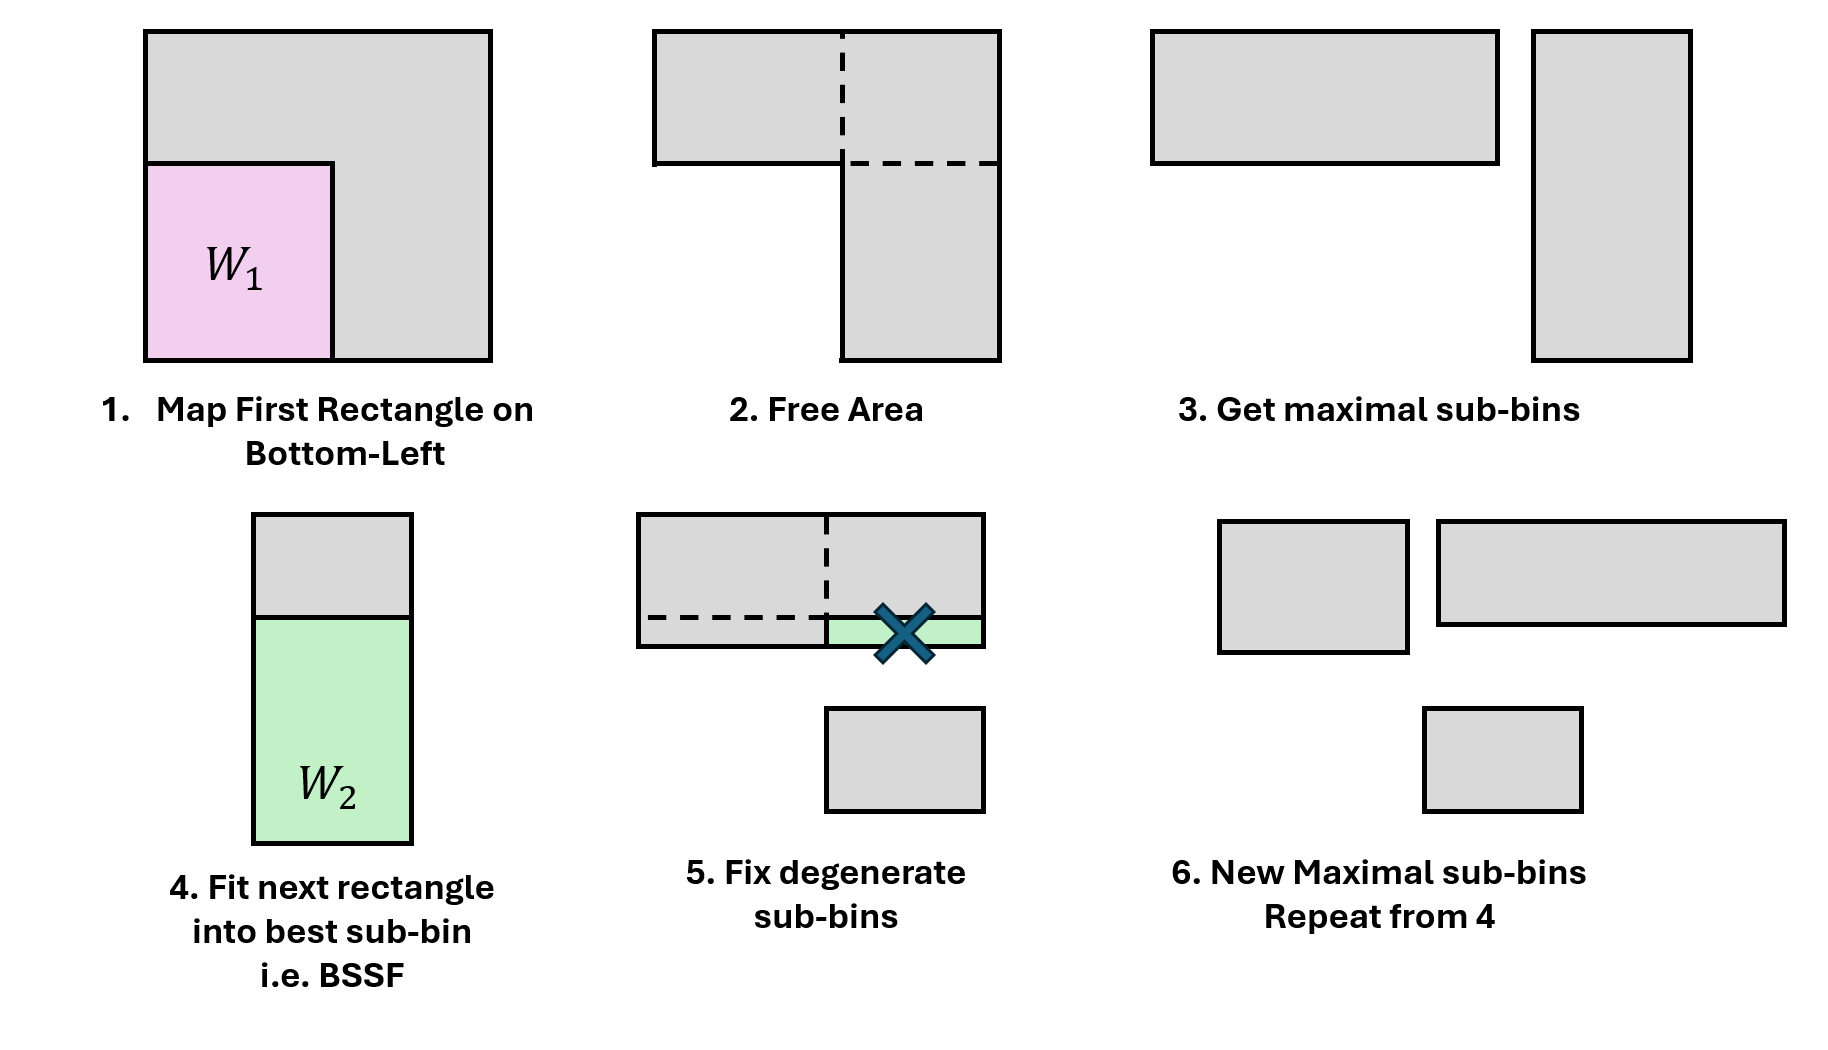
\includegraphics[width=\textwidth]{images/marp/maxrects.png}
    \caption{Maximal Rectangles algorithm. The MaxRects algorithm works by repeatedly placing new rectangles into the remaining overlapping empty rectangles of free space in a bin.}
    \label{fig:maxrects}
\end{figure}

As we'll mostly be using the MaxRects algorithm, we will briefly explain how it works. Figure \ref{fig:maxrects} shows a compact explanation of the MaxRects algorithm. First, we place a rectangle on the bottom-left corner of the empty bin (widely considered the best first move). With this placement, we create an L-shaped free space region. This free space region can always be split into two smaller overlapping rectangles which are "maximal"- that is, they are the largest possible free space rectangles in at least one dimension. We can call these new free space rectangles the "maximal sub-bins". We then consider the new free space rectangles as new bins. Using one of the fitting heuristics shown in Figure \ref{fig:maximal_rectangles_variants}, we can then place the next rectangle into one of the maximal sub-bins. For example, if we use the "Best Short Side Fit" (BSSF) heuristic, we will place the next rectangle into the maximal sub-bin that has the shortest side that can fit the rectangle. This process is repeated until all rectangles are placed or no more rectangles can be placed. Explanations on the other rectangular packing algorithms (SkyLine, Guillotine) can be found in Jylanki's paper \cite{jylanki2010thousand}. 

\subsection{Binning}

\begin{figure}[htbp]
    \centering
    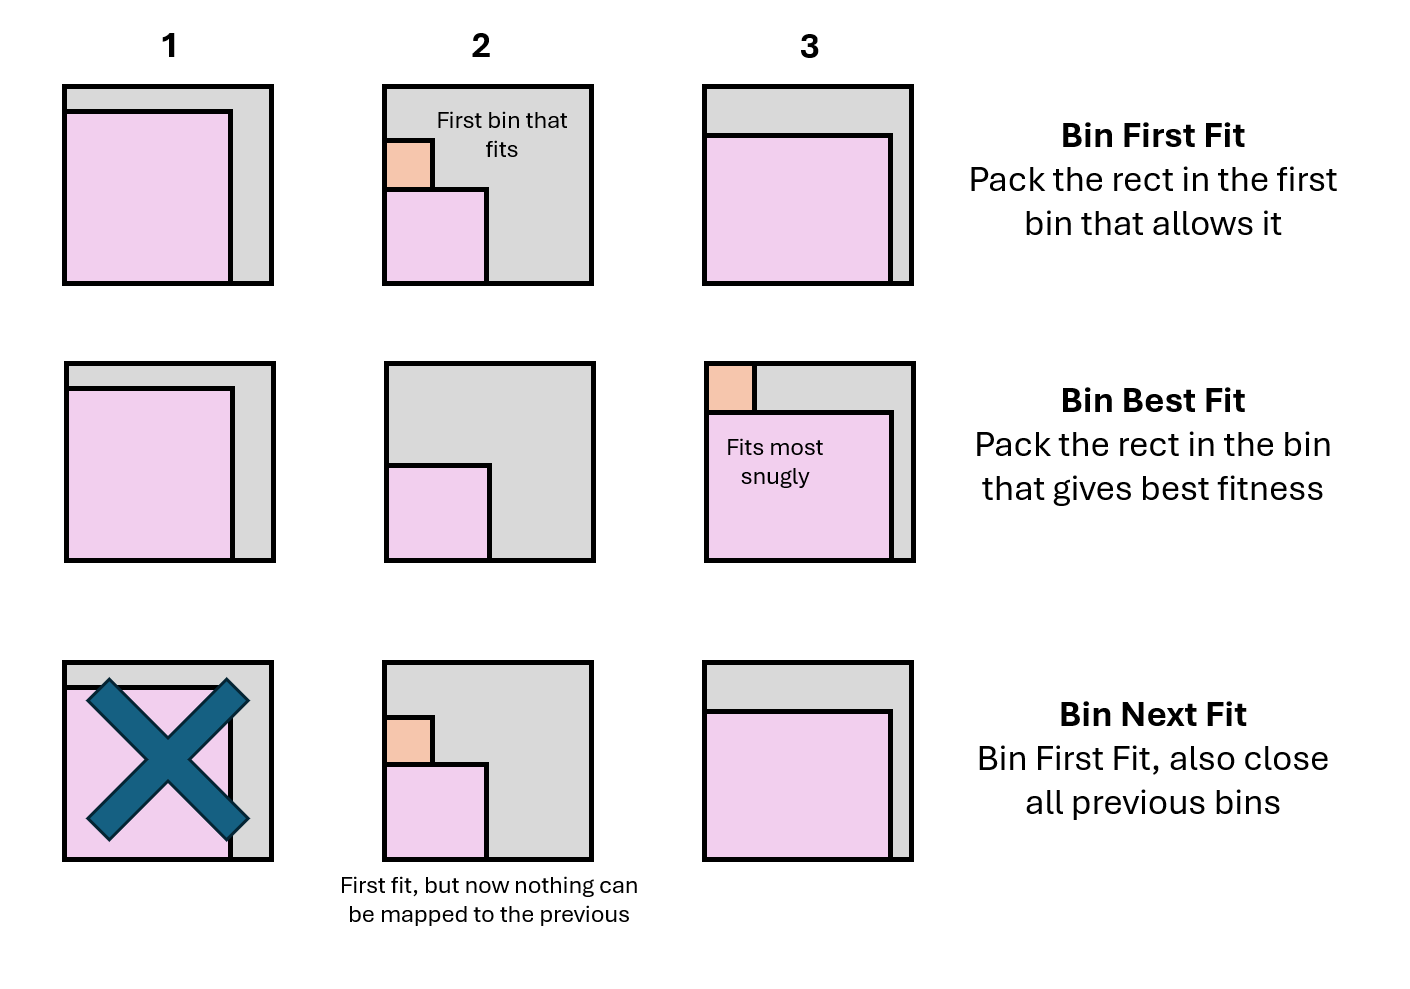
\includegraphics[width=\textwidth]{images/marp/binning.png}
    \caption{Binning heuristics.}
    \label{fig:binning}
\end{figure}

When we need to pack multiple rectangles into multiple bins, we can use the same MaxRects algorithm in combination with a binning heuristic. The binning heuristic determines how the rectangles are placed into the bins, as shown in Figure \ref{fig:binning}. The bin first fit (BFF) heuristic places the rectangles into the first bin that has enough space for the rectangle. If no bins are able to fit the rectangle, a new bin is created. The bin best fit (BBF) heuristic places the rectangle into the bin that has the best fitting heuristic score (as in BSSF, like before) for the rectangle. Lastly, the bin next fit (BNF) heuristic is exactly the same as BFF, but it closes bins after they reject a rectangle. This means that even if the next rectangle could fit in a previous bin, it will not be placed in that bin.

\subsection{Offline and Online Packing}

More than a heuristic, offline and online packing are variations of the rectangular packing problem. Offline packing is when all the rectangles are known beforehand and can be packed into the bins in a single pass. In that case, we can sort the rectangles beforehand (typically by longest side) before packing. This typically results in very dense packings. Online packing is when the rectangles are not known beforehand and can only be packed into the bins as they arrive. In that case, we cannot sort the rectangles beforehand and must pack them in the order they arrive. This typically results in less dense packings, but as we will see later, it results in less overall writes and more bin reuse in the context of DNN mappings.

\section{Splitting ONNX Models}

\begin{figure}[htbp]
    \centering
    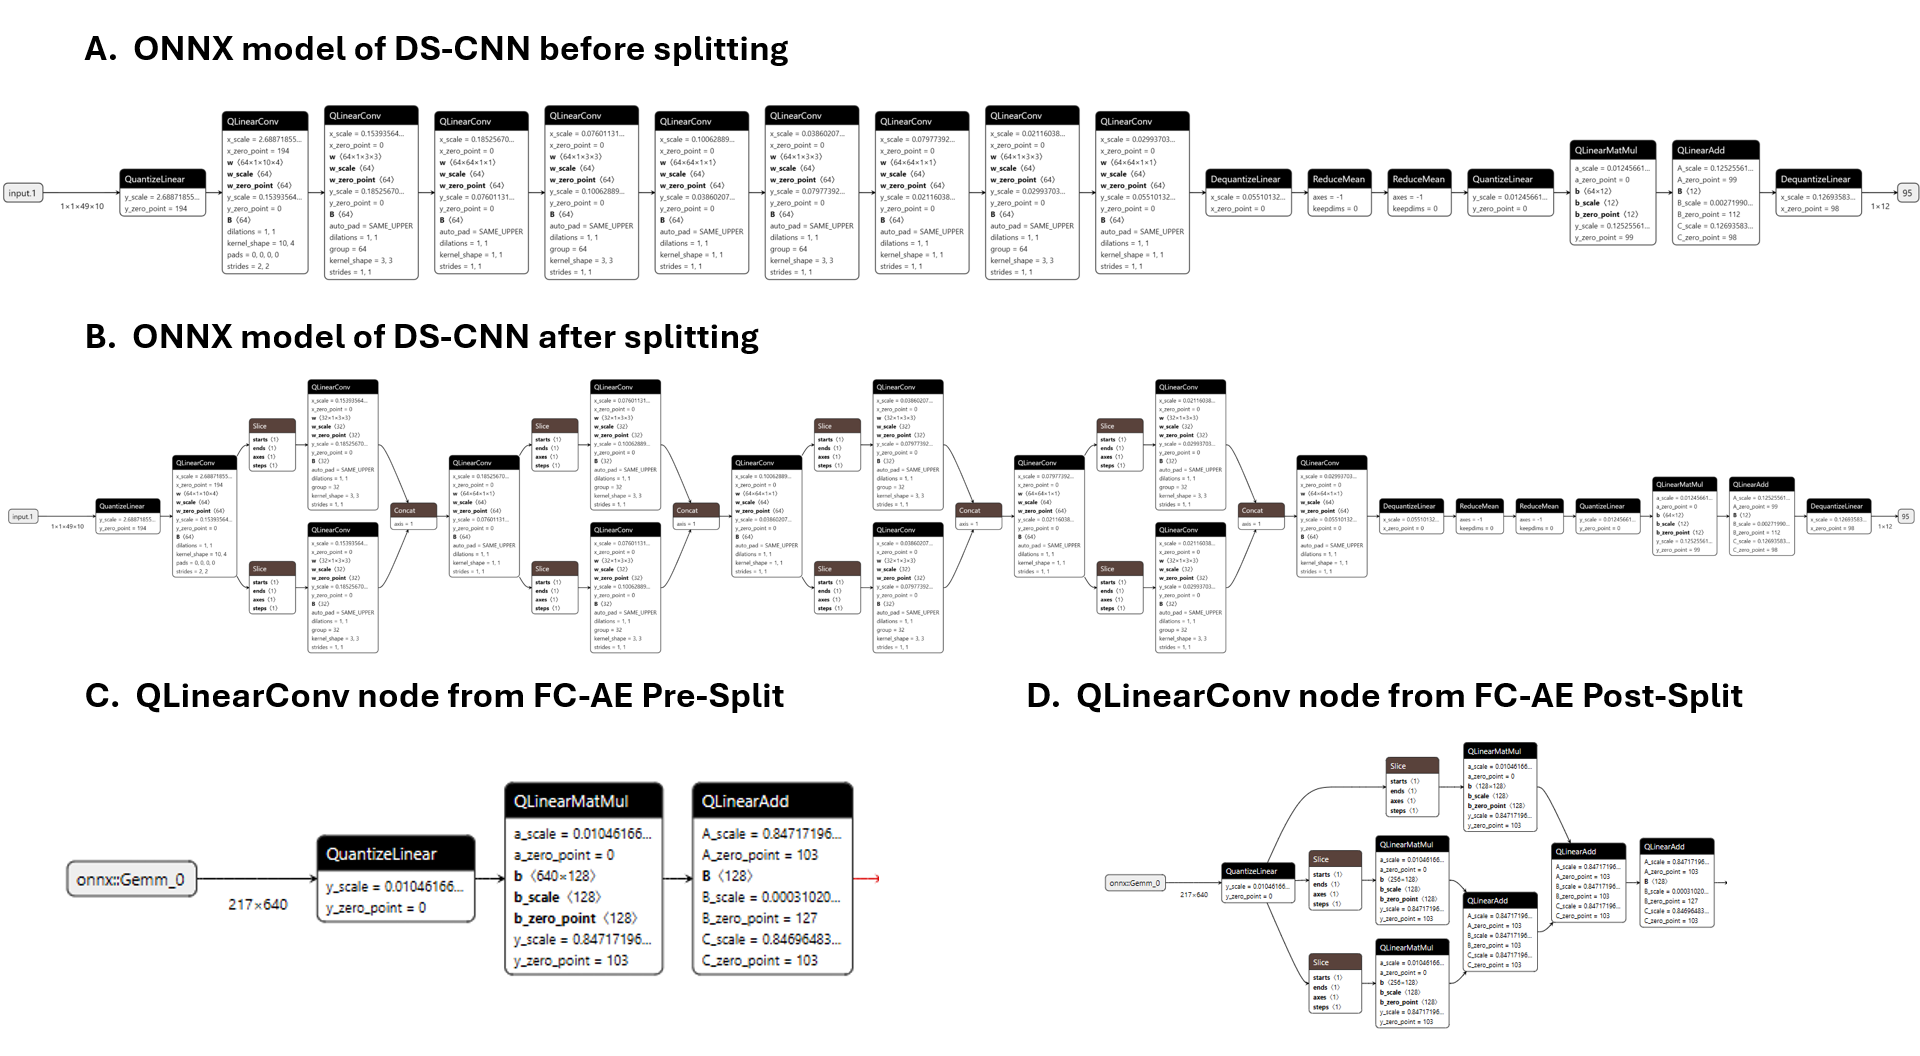
\includegraphics[width=\textwidth]{images/marp/onnx_and_splitting.png}
    \caption{(A) ONNX Graph for the Keyword Spotting DS-CNN. (B) ONNX Graph for DS-CNN after splitting. (C) First few layers of the FC-AE graph. (D) First few layers of the FC-AE graph after splitting. }
    \label{fig:onnx}
\end{figure}

In order to work with DNN models, MARP uses the ONNX format \cite{onnxruntime}. We find that it's easiest to work with ONNX models in hardware if they are represented as computational graphs. Figure \ref{fig:onnx}A shows the ONNX graph of MLPerfTiny's DS-CNN model for keyword spotting.

When mapping an ONNX model, MARP needs to split the model into layers that can fit into the corresponding hardware. Because QRAcc (Chapter \ref{chap:qracc}) can only map matrices that are at most 256x256, MARP splits large non-depthwise convolution layers into layers with at most $K=256$ and $C*F_X*F_Y=256$. For depthwise convolution layers, MARP splits them into layers with at most $C=32$ as QRAcc's digital accelerator can only support depthwise convolutions with at most 32 channels. Figure \ref{fig:onnx}B shows the ONNX graph of the DS-CNN model after splitting all of the depthwise layers into layers with at most 32 channels. As another example, Figure \ref{fig:onnx}C shows the first few layers of the FC-AE model for anomaly detection on ToyADMOS. The first MatMul layer of FC-AE is too large to fit into QRAcc's 256x256 AIMC memory array, so MARP splits them into three layers with $K=[256,256,128]$. Figure \ref{fig:onnx}D shows the first few layers of the FC-AE model after splitting the first MatMul layer into three layers with $K=[256,256,128]$. 

When layers are split C-wise (over the input channels), MARP needs to add a slice node before the split layer and an add node after the split layer. The slice node allows the next layer to get the appropriate set of input channels that it's meant to process, while the add node puts together partial sums that are supposed to result in the same output channel. When layers are split K-wise (over the output channels), MARP needs to add a concatenate node after the split layer. The concatenate node allows multiple sets of tensors to be concatenated together to form the final output tensor to form the original K output channels. 

\section{Compiling Nodes for Hardware}

MARP extracts the layer information from each node of the ONNX model and places it into a custom data structure called \texttt{MappedQRAccNode}. A \texttt{MappedQRAccNode} contains all the original information of the layer, but also the Bin ID of the bin that the layer is mapped to, the Offset X and offset Y which are the offsets of the layer in the bin, and the changed scales, biases, and offsets of the QLinear node for integer-only convolutions (explained in Chapter \ref{section:qlinearops}).

MARP then compiles the \texttt{MappedQRAccNode} into a set of CSR writes for the accelerator. The CSR writes are the control and status registers (CSRs) that the accelerator (here, QRAcc) uses to configure itself to run a layer. MARP also generates the input feature map writes and weight writes if needed for the layer. We use an intermediate representation that is not necessarily assembly for testing the compilation. However, we believe compilation targeting a specific processor instruction set architecture should be easy to implement in an almost one-to-one manner. 

MARP also implements a traversal function of the mapped ONNX graph, which is used to traverse the graph in a topological order i.e. in order of execution. Using this graph traversal, MARP can discover and optimize dependencies between succeeding layers. We list MARP's compilation optimizations as follows:

\begin{itemize}
    \item \textbf{Ifmap Reuse:} If the currently loaded Ifmap in the accelerator is the same as the Ifmap of the next layer, MARP can skip writing the Ifmap to the accelerator and use that Ifmap for the next layer. This is useful for layers that have the same Ifmap, such as depthwise convolutions.
    \item \textbf{Ofmap Ping-Pong:} If the previous layer's Ofmap is the same as the next layer's Ifmap, MARP can skip reading the Ofmap from the accelerator and use the previous layer's Ofmap as the next layer's Ifmap. This is the most common case in DNNs, as most layers have the previous layer's Ofmap as their Ifmap.
    \item \textbf{Weight Bin Reuse:} If the next layer's weights are mapped into the same bin as the previous layer's weights, MARP skips writing the weights to the accelerator and instead just changes the offset configuration, biases and scales loaded in the accelerator.
    
\end{itemize}

MARP's compilation algorithms can be found in \url{https://github.com/Lawrence-lugs/hwacc_design_garage/blob/main/hwacctools/comp_graph/core.py} and \url{https://github.com/Lawrence-lugs/QrAccelerator/blob/main/tests/stim_lib/compile.py}.

\section{Results}

\subsection{Three Optimal Subtypes of MaxRects}

\begin{figure}[htbp]
    \centering
    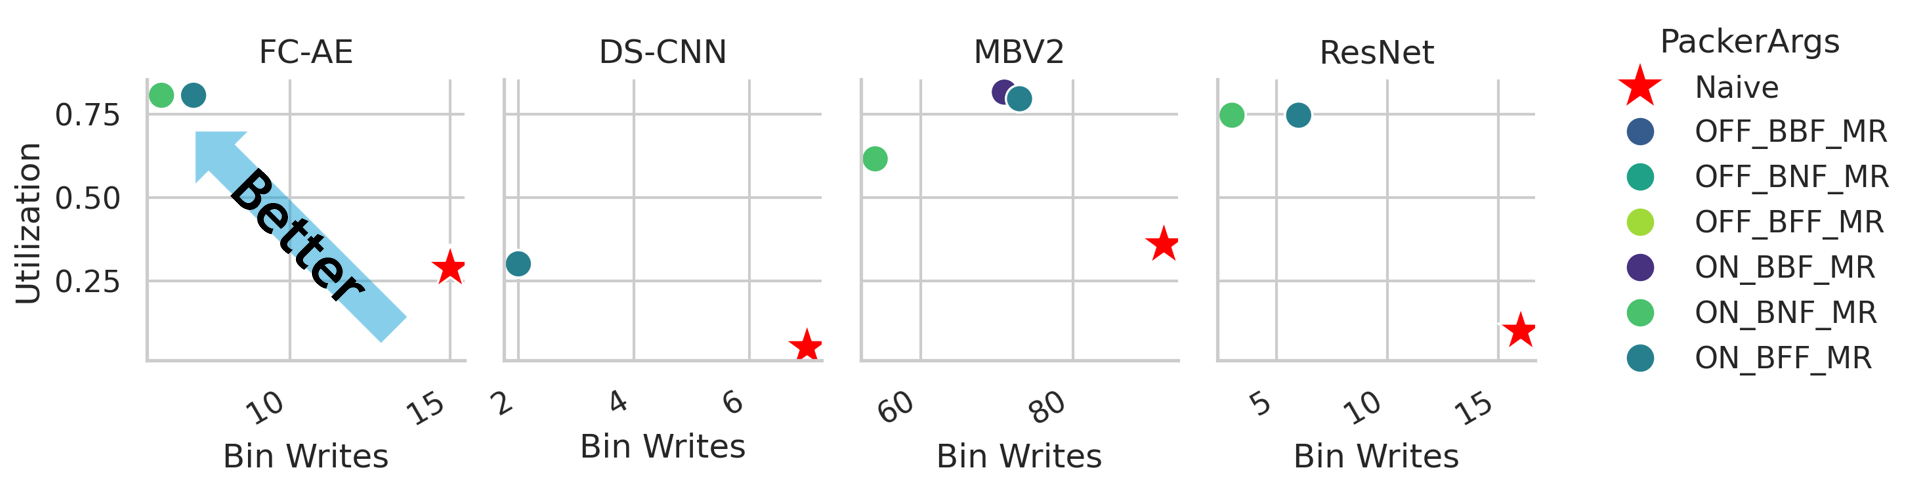
\includegraphics[width=\textwidth]{images/marp/mlperftiny_packers.png}
    \caption{Utilization vs Bin Writes of the MLPerfTiny models for various variants of the MaxRects (MR) algorithm. Different rectpack variants trade off utilization for bin writes, but using rectangular packing always improves both compared to single-mapping.}
    \label{fig:mlperftiny_packers}
\end{figure}


\begin{figure}[htbp]
    \centering
    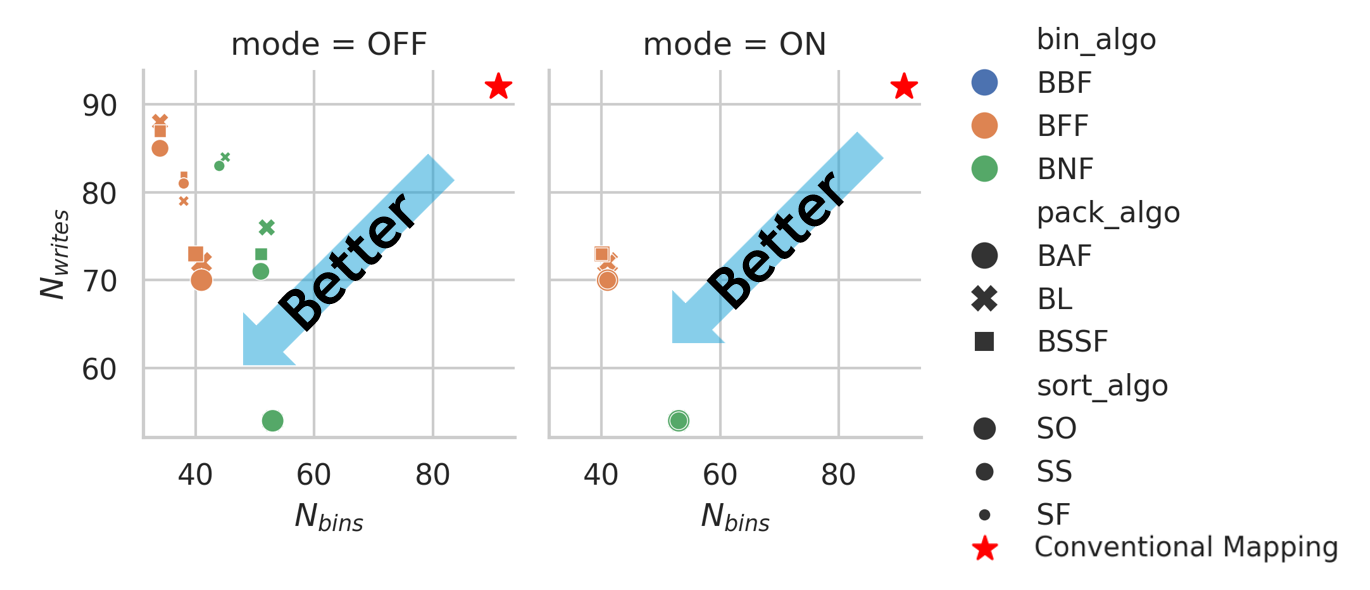
\includegraphics[width=0.8\textwidth]{images/marp/bssf_types.png}
    \caption{Utilization vs Bin Writes of the MBV2 for even more variants of the MaxRects algorithm.}
    \label{fig:bssf_types}
\end{figure}

We performed preliminary experiments to compare the performance of different MaxRects packers on the MLPerfTiny models. Figure \ref{fig:mlperftiny_packers} shows the performance of the different packers on the MLPerfTiny Models. It is visible that the naive single-mapping packer achieves the worst utilization and the most bin writes for any given model. Figure \ref{fig:bssf_types} shows our experiments on more variants of the MaxRects algorithm on the MobileNetV2 model. 

\begin{table}[h]
\caption{Results of the 4 main packers on the MLPerfTiny models on a 256x256 core size}
\label{table:marp_on_mlperftiny}
\centering
\begin{tabular}{ccccc}
\hline
\textbf{Model} & \textbf{Packer} & \textbf{Utilization} & \textbf{Bin Writes} & \textbf{\# Bins} \\ \hline
\multirow{4}{*}{DS-CNN} & Naive          & 5.01\%           & 7           & 6           \\ \cline{2-5} 
                        & Dense          & \textbf{30.08\%} & \textbf{2}  & \textbf{1}  \\
                        & Balanced       & \textbf{30.08\%} & \textbf{2}  & \textbf{1}  \\
               & WriteOptimized  & \textbf{30.08\%}     & \textbf{2}          & \textbf{1}       \\ \hline
\multirow{4}{*}{FC-AE}  & Naive          & 28.79\%          & 15          & 14          \\ \cline{2-5} 
                        & Dense          & \textbf{80.63\%} & 7           & 5           \\
                        & Balanced       & \textbf{80.63\%} & 7           & 5           \\
                        & WriteOptimized & \textbf{80.63\%} & \textbf{6}  & 5           \\ \hline
\multirow{4}{*}{MBV2}   & Naive          & 35.86\%          & 92          & 91          \\ \cline{2-5} 
                        & Dense          & \textbf{81.57\%} & 71          & \textbf{40} \\
                        & Balanced       & \textbf{81.57\%} & 71          & \textbf{40} \\
                        & WriteOptimized & 61.56\%          & \textbf{54} & 53          \\ \hline
\multirow{4}{*}{ResNet} & Naive          & 9.95\%           & 16          & 15          \\ \cline{2-5} 
                        & Dense          & \textbf{74.65\%} & 6           & \textbf{2}  \\
                        & Balanced       & \textbf{74.65\%} & 6           & \textbf{2}  \\
                        & WriteOptimized & \textbf{74.65\%} & \textbf{3}  & 2          
\end{tabular}
\end{table}

We find that in terms of bin writes, most of the offline packers (the ones with OFF) achieve roughly the same max utilization while trading off bin writes. The "Offline-Bin Best Fit" (OFF-BBF) configuration achieves the best utilization with the least bin writes. We call this configuration the "Dense" configuration. The "Online-Bin Next Fit" (ON-BNF) configuration tends to achieve the least bin writes at a less dense packing. We call this configuration the "Write-Optimized" configuration. The "Online-Bin Best Fit" (ON-BBF) configuration achieves a good balance between utilization and bin writes, so we call this configuration the "Balanced" configuration. Table \ref{table:marp_on_mlperftiny} summarizes the results of the 4 main packers on the MLPerfTiny models.

\begin{figure}[htbp]
    \centering
    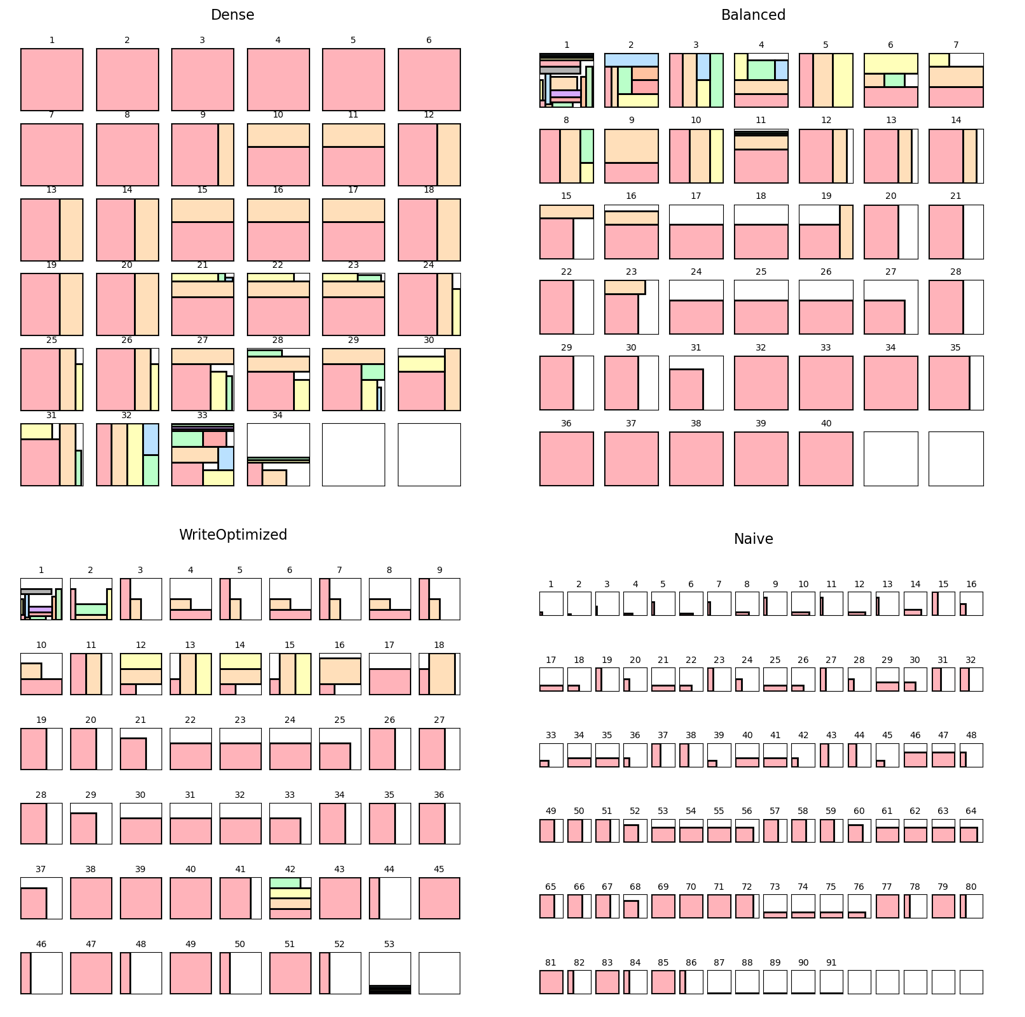
\includegraphics[width=\textwidth]{images/marp/mbv2_sample.png}
    \caption{Sample mappings of the 4 packer configurations of MobileNetV2 on a 256x256 core size}
    \label{fig:mbv2_sample}
\end{figure}

Sample packings of the 4 configurations (including Naive) are shown in Figure \ref{fig:mbv2_sample}.

\subsection{Access Patterns}

\begin{figure}[htbp]
    \centering
    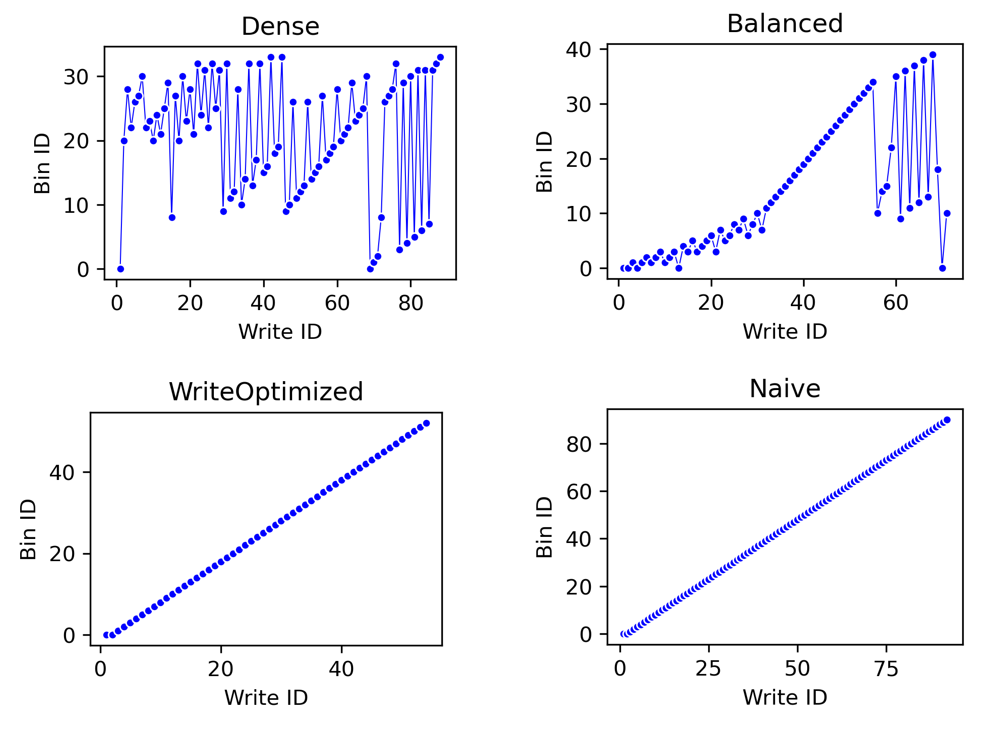
\includegraphics[width=\textwidth]{images/marp/mbv2_access_patterns.png}
    \caption{Access patterns on MobileNetV2 of the different packers}
    \label{fig:mbv2_access_patterns}
\end{figure}

To show the reason why the different packers achieve different numbers of bin writes, we show the access patterns of the MobileNetV2 model under MARP in Figure \ref{fig:mbv2_access_patterns}. The Dense packer, which works offline, has global information about all the layers (rectangles) at the same time and so it can pack each layer anywhere regardless of order. This results in the most dense packing, but it results in each successive layer (Write ID) being almost guaranteed to have a different bin. For the Balanced packer, it is an online packer which means it has to pack each layer as they arrive (as sorted in the execution order). However, due to the BBF binning heuristic, it can still pack the layer into previous bins if it is a better fit. This causes backtracking to previous bins in the access patterns. The Write-Optimized packer is also an online packer, but it uses the BNF binning heuristic which does not allow backtracking to previous bins. This results in more bins being created, but also guarantees that each successive layer will either be in the same bin as the previous layer or in the next bin. Lastly, the Naive packer has a similar access pattern to the Write-Optimized packer, but that's only because it packs each layer into a separate bin and hence the bins can be accessed in order. 

\section{Conclusion}

In this chapter, we presented MARP, a DNN mapper that can optimize the mapping of multiple layers in AIMC accelerators with interlayer weight reuse. We showed that MARP can increase the utilization of the MLPerfTiny models by packing multiple layers into a single AIMC memory array using rectangular packing algorithms. We also showed that MARP can reduce the number of AIMC cores needed to fully map models by packing multiple layers into a single AIMC memory array.

Mappings with very low bin writes are ideal for AIMC accelerators like QRAcc with a single core. AIMC accelerators like NeuRRAM with more cores can benefit more from using the densest packings as they can simultaneously load multiple bins into different cores. 

In the next chapter, we will present QRAcc, a hybrid AIMC accelerator that can run depthwise convolutions efficiently by using a weight-stationary digital accelerator. QRAcc was codesigned with MARP in mind, so it can take advantage of the optimizations that MARP provides.